\chapter{URLs for Content in eXpressive Internet Architecture}
\label{sec:urls}

\section{Universal Resource Locators (URLs)}
The resources in the world wide web are identified by
\textbf{Universal Resource Identifier} often acronymed as
\textbf{URIs}. URIs allow identifying resources uniquely thus giving
hosts the ability to express interest in specific resources. The most
common form of URIs is \textbf{Universal Resource Locators or
  URLs}. URLs, in addition to uniquely identifying a resource also
specifies a mechanism to retrieve the resource. The URLs in general
look like the following:

\begin{center}
  \textbf{\textit{protocol}://\textit{host}/\textit{path}}
\end{center}

The \textit{protocol} field specifies the scheme that should be used
to retrieve a representation of the resource. The most popular
resource retrieval scheme in the web is `HTTP'. Other possible schemes
are `FTP', `file', `data'. The \textit{host} part is the network
location of the resource. It can be an IPv4 address or a domain name
that the DNS can resolve to an IPv4 address. A \textit{host} can own
multiple resources. The \textit{path} is the specific location of the
resource on the \textit{host}.

\section{URL Design Goal}
The goals of URL design for CIDs and nCIDs are two-fold.

Firstly, the web resources refer to other web resources all the
time. For example, the HTML web pages contain URLs of other web
resources. In the previous chapters we have seen that the CIDs can be
used better to represent static web resources. On the other hand,
nCIDs are a better fit for multiform resources. Since, in this thesis
we use CIDs and nCIDs to represent web resources, we need a method of
pointing to these web resources.

Secondly, the advantage that nCIDs have over the CIDs is that they are
addressable by human readable names. Hence, constructing nCID URLs is
a fairly understood problem. But the goal of URL design for CIDs is
that the constructed URLs should be able to directly refer to the
content avoiding name lookups.


\section{URLs for CIDs}
\label{sec:urlcid}
We propose following format for CID URLs.
\begin{center}
  \textbf{\textit{cid}://\textit{serialized-cid-dag}}
\end{center}
In order to understand the process of DAG serialization, let us take
an example of a CID DAG address as shown in \ref{fig:cid_dag}.

\begin{figure}
  \begin{center}
    \label{fig:cid_dag}
    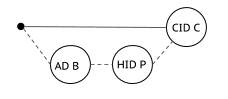
\includegraphics[scale = 0.75]{cid_dag_publisher}
    \caption{An example CID DAG address}
  \end{center}
\end{figure}

We follow the following process to make a serialized version of the
DAG:
\begin{enumerate}
  \item{Number all the nodes starting with zero and excluding the
    source node.}
  \item{List all the nodes in the order they are numbered from zero to
    maximum.}
  \item{For each node, associate the destination node number for all
    the \textit{outgoing} edges from that node.}
  \item{Prepend the output of the last step with the outgoing edges
    from the source node.}
\end{enumerate}

\begin{figure}
  \begin{center}
  \label{fig:cid_dag_serialization}
  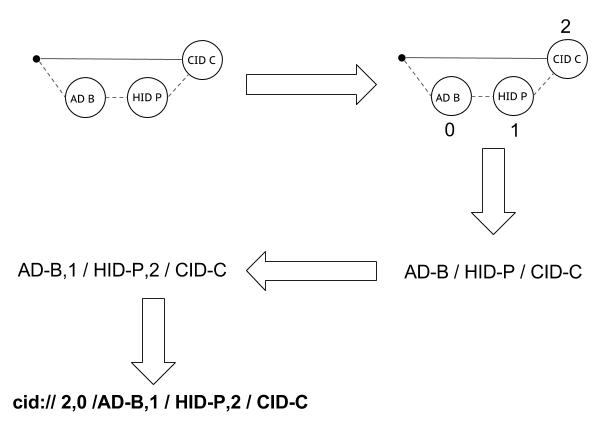
\includegraphics[scale=0.75]{dag_serialization}
  \caption{CID DAG Serialization}
  \end{center}
\end{figure}

This scheme results in an URL for CIDs that looks like this
\begin{center}
  \textbf{cid://2,0/AD-B,1/HID-P,2/CID-C}
\end{center}
The URLs that are created by this scheme are highly expressive. You
can see that \emph{any} DAG can be expressed by this method. That
allows us to use protocols other than CIDs too. For example, we could
create an URL for representing a service S as follows.
\begin{center}
  \textbf{\emph{sid}://2,0/AD-B,1/HID-P,2/\emph{SID}-S}
\end{center}
These URLs, since they directly address the content, avoid name lookup
completely. With these URLs we can now represent static resources in
the web.

\section{URLs for nCIDs}
We could readily use the URL scheme that we discussed in section
\ref{sec:urlcid}. But, the disadvantage of such an approach is that
the URLs created are highly unreadable. Since nCIDs are directly
derived from human readable names, we define a URL scheme which
results in URLs as we see today and yet avoids the need of name
look-ups completely.

\subsection{Addresses and Locators}
\label{sec:addrnloc}
We have seen that nCIDs are most useful for representing the multiform
web resources. The peculiar characteristic of multiform resources is
that they change their form based on certain \emph{attributes}. In
essence, all the representations of the same resource share the same
\emph{address} but are uniquely identified when the address is coupled
with the \emph{attributes}. We call the attributes that locate a
certain representation of a resource the \emph{locators}.\\
As a motivating example, let's take a case of multiform resources
identified by URL \emph{http://wikipedia.org/google}. It is easy to
see that when this web resource is requested from a desktop it takes a
certain representation. While the same resource, if requested from a
mobile device, takes a completely different form. So, even though the
two objects are totally different in terms of their content, they do
share an identity. This identity is their address. To sum up,
address of a multiform resource allows us to identify a resource and
locators help us locate a representation of the resource.

\begin{figure}
\begin{center}
  \label{fig:multiform-change}
  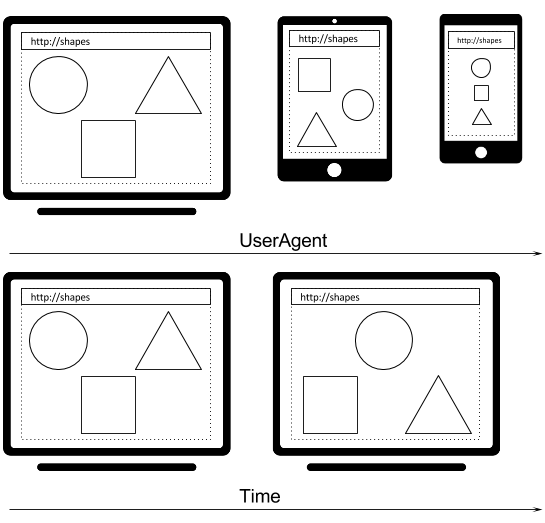
\includegraphics[scale=0.75]{multiform_changing_form}
  \caption{Multiform resource changing its form}
\end{center}
\end{figure}

\subsection{nCID URL Design}
Based on the learning from section \ref{sec:addrnloc}, we propose the
following format for the URLs of nCIDs.
\begin{center}
  \textbf{ncid://address/locator1=value1\&locator2=value2\&...}
\end{center}
With respect to the motivating example shown in figure
\ref{fig:multiform-change}, the address of the content is
\emph{content.facebook.com} whereas an locator is
\emph{UserAgent=Android}. Table \ref{tab:locators} shows the list of
possible locators. Our security model enforces us to mandate either
the implicit or the explicit existence of a locator called
\emph{certificate}. The locator \emph{certificate} is essentially the
pointer to the public key certificate that would be used to verify
authenticity and integrity of the named content chunk.

\begin{table}
  \begin{center}
    \begin{tabular}
      {c | c | c}
      Name & Details & Mandatory \\
      \hline
      PubCert & DAG Address of the Publisher's Public Key Certificate & Yes \\
      Version & Version of the Content Chunk & No\\
      UserAgent & HTTP UserAgent & No\\
    \end{tabular}
    \label{tab:locators}
  \end{center}
  \caption{List of Locators}
\end{table}

\section{Conclusion}

In this chapter, we defined URL schemes for CID and nCID type content
chunks. With CID URLs, we provided a way to point to CID chunks while
avoiding name lookups. The nCID URL scheme allows us effectively
express a link to a nCID resource. Separating addresses and locators
gives web users the ability to choose specifically the representation
that suites its needs the best.

